{\Large Papai Noel não existe, nem coelhinho da pascoa!}

{\Large Usuário: o negacionista da Ciência de Computação.}


\vfill\null
\columnbreak

\begin{center}
	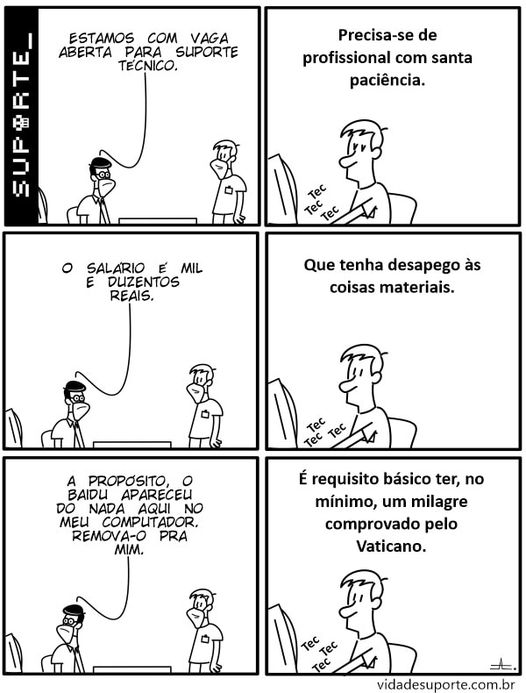
\includegraphics[height=\textheight]{./IMG/TI.jpg}
\end{center}

\begin{center}
	
\includegraphics[width=\linewidth]{./IMG/usuario.jpg}
\end{center}


\large
\label{link1}
\href{http://www.link1.com}{Link 1}


\begin{enumerate}
	\item Computação e mercado de trabalho.
	\item Nunca duvide da capacidade do usuario!
	\item O carinha do TI
	\item Programador
	\item A segurança
	\item Custos
	\item Projeto de vida
\end{enumerate}

crie um roteiro para uma serie de videos curtos, explicando para usuarios os principais golpes na internet e como evita-los 

Vídeo 1: Introdução aos golpes na internet - Explicar o que são golpes na internet e como eles funcionam.

Vídeo 2: Golpe do phishing - Explicar o que e phishing e como os golpistas se passam por empresas confiaveis para obter informacões pessoais. Fornecer exemplos de e-mails de phishing e mostrar como identifica-los.

Vídeo 3: Golpe do vírus - Explicar como os vírus podem ser disseminados através de e-mails ou arquivos baixados e como evitar esses golpes.

Vídeo 4: Golpe do cartao de credito - Explicar como os golpistas podem obter informacões de cartao de credito e como proteger suas informacões financeiras.

Vídeo 5: Golpe de investimento - Explicar como os golpistas podem se passar por corretores de investimentos confiaveis e como evitar esses golpes.

Vídeo 6: Conclusão - Revisar os principais golpes na internet e fornecer dicas gerais sobre como se proteger.

aravecchia@gmail.com
detalhe o video 1

Vídeo 1: Introdução aos golpes na internet

Título: "Fique atento: Conheca os principais golpes na internet"

Duração: aproximadamente 5-7 minutos

Introdução: Explicar o objetivo do vídeo e o que sera abordado. Informar que os golpes na internet estão se tornando cada vez mais comuns e e importante estar ciente deles para se proteger.

Definição de golpes na internet: Explicar o que são golpes na internet e como eles funcionam. Fornecer exemplos de golpes comuns, como phishing, vírus, golpes de cartao de credito e golpes de investimento.

Metodos de ataque: Explicar como os golpistas usam tecnicas de engenharia social para obter informacões pessoais e financeiras. Mostrar exemplos de e-mails e mensagens de texto de golpes, bem como sites falsos que se parecem com sites legítimos.

Conselhos de segurança: Fornecer dicas gerais sobre como se proteger dos golpes na internet, como manter seu software de segurança atualizado, não clicar em links suspeitos, não fornecer informacões pessoais a não ser que você confie na fonte e ser desconfiado de ofertas que parecem boas demais para ser verdade.

Conclusão: Concluir o vídeo enfatizando a importancia de estar ciente dos golpes na internet e seguir as dicas de segurança para se proteger. Informar que os próximos vídeos irao se aprofundar em golpes específicos e como evita-los.

aravecchia@gmail.com
detalhe o video 2

Vídeo 2: Golpe do phishing

Título: "Como se proteger do phishing: entenda o golpe e saiba como evita-lo"

Duração: aproximadamente 5-7 minutos

Introdução: Explicar o objetivo do vídeo e o que sera abordado. Informar que o phishing e um dos golpes mais comuns na internet e e importante estar ciente dele para se proteger.

Definição de phishing: Explicar o que e phishing e como os golpistas se passam por empresas confiaveis para obter informacões pessoais. Fornecer exemplos de e-mails de phishing, como solicitacões de senha ou informacões de cartao de credito.

Identificando e-mails de phishing: Mostrar como identificar e-mails de phishing, como erros de ortografia, URLs suspeitos e solicitacões de informacões pessoais. Explicar a importancia de não clicar em links ou fornecer informacões pessoais sem antes verificar a veracidade da fonte.

Conselhos de segurança: Fornecer dicas gerais sobre como se proteger do phishing, como não clicar em links suspeitos, não fornecer informacões pessoais a não ser que você confie na fonte, usar ferramentas de segurança como filtros de spam e ser desconfiado de e-mails que parecem estranhos.

Conclusão: Concluir o vídeo enfatizando a importancia de estar ciente do phishing e seguir as dicas de segurança para se proteger. Informar que os próximos vídeos irao se aprofundar em outros golpes específicos e como evita-los.

aravecchia@gmail.com
detalhe o video 3

Vídeo 3: Golpe do vírus

Título: "Não caia na armadilha: Como se proteger dos vírus na internet"

Duração: aproximadamente 5-7 minutos

Introdução: Explicar o objetivo do vídeo e o que sera abordado. Informar que os vírus na internet são uma ameaca real e e importante estar ciente deles para se proteger.

Definição de vírus: Explicar o que são vírus e como eles podem ser disseminados através de e-mails ou arquivos baixados. Fornecer exemplos de vírus comuns, como vírus de ransomware, vírus de Trojan e vírus de spyware.

Identificando vírus: Mostrar como identificar vírus, como mensagens de erro estranhas, lentidao do computador e pop-ups suspeitos. Explicar a importancia de manter seu software de segurança atualizado e usar um firewall para se proteger.

Conselhos de segurança: Fornecer dicas gerais sobre como se proteger dos vírus, como não abrir e-mails ou arquivos suspeitos, não clicar em links suspeitos, manter seu software de segurança atualizado e fazer backup de seus arquivos importantes.

Conclusão: Concluir o vídeo enfatizando a importancia de estar ciente dos vírus na internet e seguir as dicas de segurança para se proteger. Informar que os próximos vídeos irao se aprofundar em outros golpes específicos e como evita-los.

aravecchia@gmail.com
detalhe o video 4

Vídeo 4: Golpe do cartao de credito

Título: "Fique alerta: Como se proteger dos golpes de cartao de credito na internet"

Duração: aproximadamente 5-7 minutos

Introdução: Explicar o objetivo do vídeo e o que sera abordado. Informar que os golpes de cartao de credito na internet são uma ameaca real e e importante estar ciente deles para se proteger.

Definição de golpe de cartao de credito: Explicar como os golpistas podem obter informacões de cartao de credito e como esses golpes funcionam. Fornecer exemplos de golpes comuns, como roubo de informacões de cartao de credito através de sites falsos, phishing e vírus.

Identificando golpes de cartao de credito: Mostrar como identificar tentativas de golpe de cartao de credito, como cobrancas suspeitas em sua conta ou mensagens de alerta de fraude. Explicar a importancia de monitorar suas contas regularmente e ficar atento a quaisquer atividades suspeitas.

Conselhos de segurança: Fornecer dicas gerais sobre como se proteger dos golpes de cartao de credito, como não fornecer informacões de cartao de credito a não ser que você confie na fonte, usar senhas fortes e protegidas, evitar compras em sites desconhecidos e usar ferramentas de segurança para proteger suas informacões financeiras.

Conclusão: Concluir o vídeo enfatizando a importancia de estar ciente dos golpes de cartao de credito na internet e seguir as dicas de segurança para se proteger. Informar que os próximos vídeos irao se aprofundar em outros golpes específicos e como evita-los.

aravecchia@gmail.com
detalhe o video 5

Vídeo 5: Golpe de investimento

Título: "Cuidado com as armadilhas: Como se proteger dos golpes de investimento na internet"

Duração: aproximadamente 5-7 minutos

Introdução: Explicar o objetivo do vídeo e o que sera abordado. Informar que os golpes de investimento na internet são uma ameaca real e e importante estar ciente deles para se proteger.

Definição de golpe de investimento: Explicar como os golpistas podem se passar por corretores de investimentos confiaveis e como esses golpes funcionam. Fornecer exemplos de golpes comuns, como ofertas de investimento falsas, esquemas Ponzi e golpes de criptomoedas.

Identificando golpes de investimento: Mostrar como identificar tentativas de golpe de investimento, como ofertas de investimento que parecem boas demais para ser verdade, promessas de retornos impossíveis, e solicitacões de investimentos de corretores desconhecidos. Explicar a importancia de fazer sua própria pesquisa antes de investir e verificar a veracidade da fonte.

Conselhos de segurança: Fornecer dicas gerais sobre como se proteger dos golpes de investimento, como fazer sua própria pesquisa antes de investir, não ceder à pressão para investir rápidamente, evitar corretores desconhecidos e não investir mais do que você pode perder.

Conclusão: Concluir o vídeo enfatizando a importancia de estar ciente dos golpes de investimento na internet e seguir as dicas de segurança para se proteger. Informar que os próximos vídeos irao se aprofundar em outros golpes específicos e como evita-los.

aravecchia@gmail.com
detalhe o video 6

Vídeo 6: Conclusão

Título: "Esteja sempre protegido: Resumo dos principais golpes na internet e dicas para se proteger"

Duração: aproximadamente 5-7 minutos

Introdução: Explicar o objetivo do vídeo e o que sera abordado. Informar que os golpes na internet estão se tornando cada vez mais comuns e e importante estar ciente deles para se proteger.

Revisão dos principais golpes: Revisar os principais golpes abordados nos vídeos anteriores, incluindo phishing, vírus, golpes de cartao de credito e golpes de investimento.

Dicas gerais de segurança: Fornecer dicas gerais sobre como se proteger dos golpes na internet, como manter seu software de segurança atualizado, não clicar em links suspeitos, não fornecer informacões pessoais a não ser que você confie na fonte, monitorar suas contas regularmente e ser desconfiado de ofertas que parecem boas demais para ser verdade.

Conclusão: Concluir o vídeo enfatizando a importancia de estar ciente dos golpes na internet e seguir as dicas de segurança para se proteger. Informar que os vídeos foram um guia para entender os principais golpes e como evita-los, e que e importante continuar atualizado e se informando para se proteger contra novos tipos de golpes.